% Created:  Mon 23 Jun 2014 13:15 PM
% @author Josh Wainwright
% File name : grid.tex

\section{Uniform Discrete Cell Method}
\label{sec:simple_grid_method}

The simplest method for analysing the distribution of points is to use a
uniform, discrete grid of cells and place the points into these cells one at a
time. Once all points have been added, the number of points that are contained
in each cell can be treated as a grey scale brightness value with lighter
pixels representing cells with more points and black cells having no points.
This gives a simple pixel image, with brightness as a function of density of
the points, in the \texttt{pnm} image format \cite{murray1996encyclopedia}. A
thresholding filter can then be applied to remove the points that are isolated
by removing the darker pixels and leave the denser areas corresponding to
clusters.

Though the resolution of this method can be easily changed by altering the size
of the cells in the grid, it performs badly when presented with data that is
even slightly noisy. If the clusters themselves have a density that is not
significantly above the background noise level, the thresholding step is prone
to either exclude much of the interesting data, or to increase the size of the
clusters by including too much noise. These two effects can be seen clearly in
Figure~\ref{fig:grid-noise}, where \texttt{palm-1.txt} is used with a cell size
of 200. The range of the data is from 0 to \num{41000} for both the $x$ and the
$y$ axes, thus the images are $\left(\rfrac{41000}{200} = \right)$ 205 by 205
pixels. This data took \SI{495}{\milli\second} to generate.

\begin{figure}[tbh]
	\centering
	\begin{subfigure}[b]{4.2cm}
		\frame{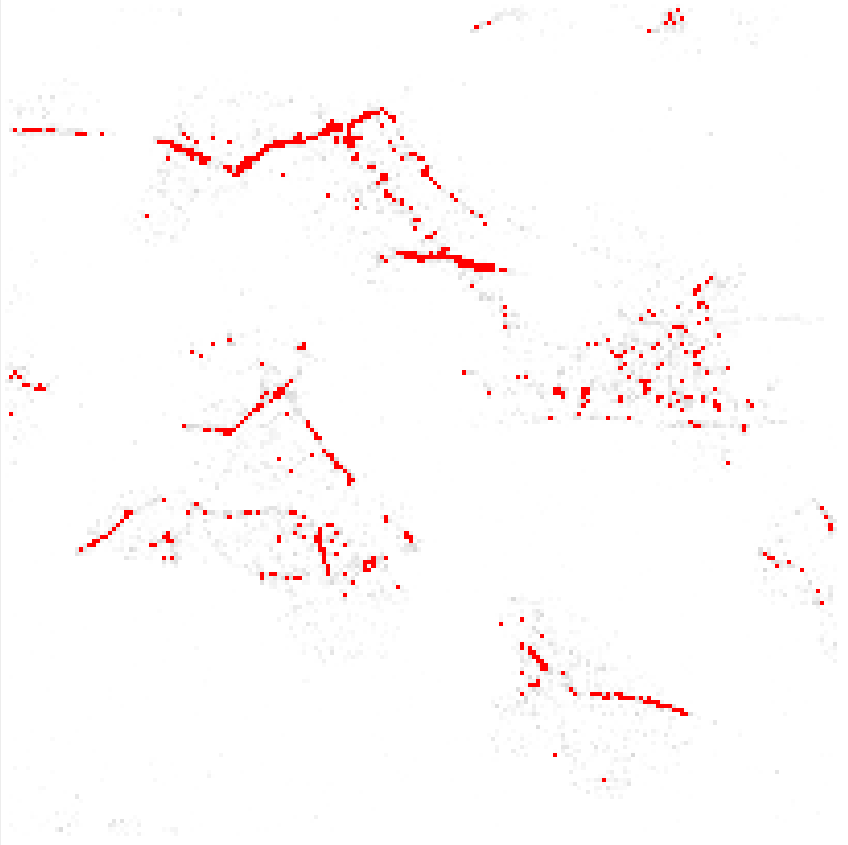
\includegraphics[width=\textwidth]{grid-noise-low.png}}
		\caption{}\label{fig:grid-noise-low.png}
	\end{subfigure}%
	\quad
	\begin{subfigure}[b]{4.2cm}
		\frame{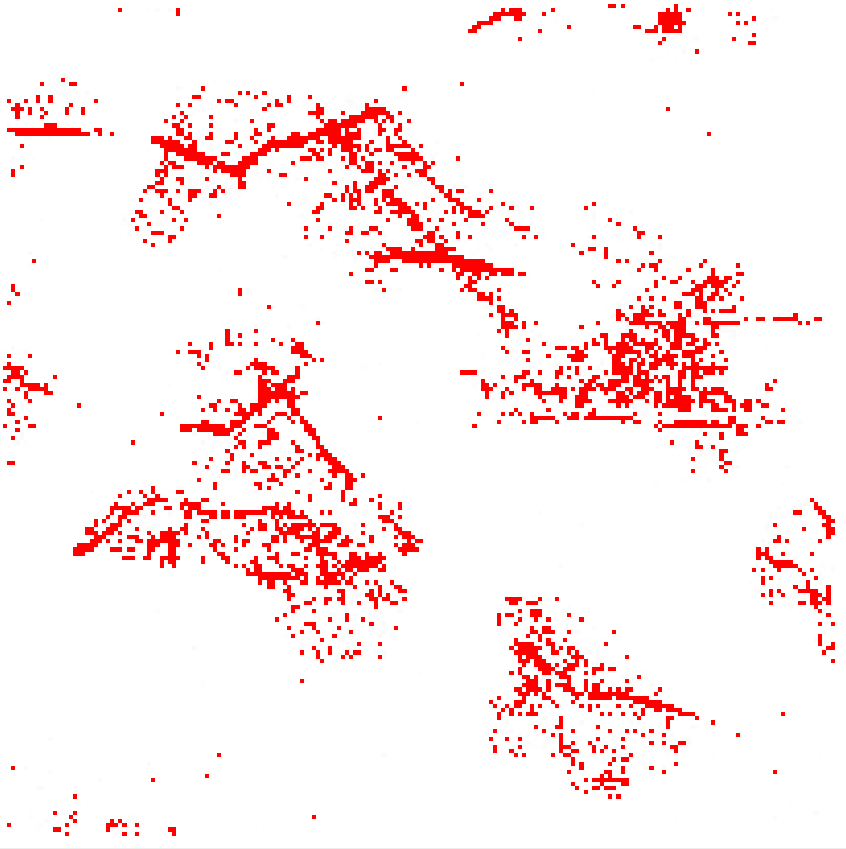
\includegraphics[width=\textwidth]{grid-noise-high.png}}
		\caption{}\label{fig:grid-noise-high.png}
	\end{subfigure}

	\caption[Effect of threshold value on clusters identified.]{Setting a low
		threshold, \subref{fig:grid-noise-low.png}, means that many of the
		points in the clusters are lost. Setting it higher,
		\subref{fig:grid-noise-high.png}, includes too many of the points
		deemed to be noise. Red pixels are ones that would be kept by the
		thresholding process, black would be removed.}\label{fig:grid-noise}
\end{figure}

There are a few steps that can be taken to improve the approach of this simple
grid when handling outlying points caused by noise:

\begin{enumerate}

	\item First, the algorithm is modified to include a thresholding step
		before writing the pixel image data to a file. This means that the
		pixels can be adjusted with greater accuracy and any arbitrary level
		can be chosen to threshold at.

	\item Next, once the image has been generated, the number of points that
		contributed to each pixel is no longer of interest and so the image can
		be converted to a binary image. This is an image with just two possible
		values. The first represents white space, where there are no points,
		the second is black where there were some number of points and so is of
		interest.

	\item Once a binary image has been generated, dilate and erode filters can
		be applied to remove remaining outliers and to try to close the gaps in
		the structures that have been identified so that they are more solid.

\end{enumerate}

\begin{figure}[tbh]
	\centering
	\frame{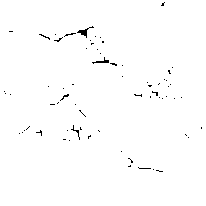
\includegraphics[width=7cm]{grid-threshold-close.png}}

	\caption[Closing algorithm to identify clusters.]{Using dilating and
		eroding algorithms can help to emphasise the structure in the
		data and, at the same time, remove the isolated points representing
		noise.}\label{fig:grid-threshold-close}
\end{figure}

These steps lead to significantly better isolation of the interesting parts of
the image, as can be seen in Figure~\ref{fig:grid-threshold-close}, however,
much of the detail of the structure is lost in this process.
